%!TEX program = xelatex
\documentclass[twoside,color=blue,mathpazo,titlestyle=hang,12pt]{elegantbook}
% \email{elegantlatex2e@gmail.com}
% \title{统计观点下的测量平差}
% \zhtitle{统计观点下的测量平差}
% \zhend{}
% \entitle{\ }
% \enend{}
% \version{2.10}
% \myquote{Victory won\rq t come to us unless we go to it.}
% \logo{logo.pdf}
% \cover{cover.pdf}

% title 
\setcounter{tocdepth}{2}
\numberwithin{equation}{section}


\title{{\Huge\emph{2018年GIS课程设计}\\实验报告}\\{\Large 项目名称:测量全生命周期支持系统}}
\author
{
\Large\textbf{同济大学测绘与地理信息学院} \\
1551126 余周炜 \\
1551140 王雪辰 \\
1551128 江子宇
}
\date{}

%green color
%    \definecolor{main1}{RGB}{0,120,2}
%    \definecolor{seco1}{RGB}{230,90,7}
%    \definecolor{thid1}{RGB}{0,160,152}

   \definecolor{main1}{RGB}{0,0,0}
   \definecolor{seco1}{RGB}{0,0,0}
   \definecolor{thid1}{RGB}{0,0,0}
%cyan color
   \definecolor{main2}{RGB}{0,175,152}
   \definecolor{seco2}{RGB}{239,126,30}
   \definecolor{thid2}{RGB}{120,8,13}
%blue color
   \definecolor{main3}{RGB}{100,149,237}
   \definecolor{seco3}{RGB}{180,50,131}
   \definecolor{thid3}{RGB}{7,127,128}

\usepackage{siunitx}
\usepackage[section]{placeins}
\usepackage{makecell}
\usepackage{listings}

\newcommand\mgape[1]{\gape{$\vcenter{\hbox{#1}}$}}

\newfontfamily\conso{Inconsolata}
\definecolor{mygreen}{rgb}{0,0.6,0}
\definecolor{mygray}{rgb}{0.5,0.5,0.5}
\definecolor{mymauve}{rgb}{0.58,0,0.82}
\lstset{backgroundcolor=\color{white},
numbers=left,
numberstyle=\small,
frame=lines,
basicstyle=\conso,
columns=fullflexible,
breaklines=true,                 % automatic line breaking only at whitespace
tabsize=4,
keywordstyle=\color{blue},
commentstyle=\color{mygreen},
stringstyle=\color{mymauve}\ttfamily,
language=Matlab}
% \usepackage[numbered,autolinebreaks,useliterate]{mcode}

% \usepackage{mdwlist}
\usepackage{lipsum}
\usepackage{colortbl}
\usepackage{texnames}
\usepackage{metalogo}
\usepackage{mflogo}
\usepackage{mathtools}
\usepackage{algorithm}
% \usepackage{algorithmicx}
\usepackage{algpseudocode}
\usepackage{longtable}
\usepackage{supertabular}
\usepackage{multirow}
\renewcommand{\algorithmicrequire}{\textbf{Input:}}  % Use Input in the format of Algorithm  
\renewcommand{\algorithmicensure}{\textbf{Output:}} % Use Output in the format of Algorithm 


\RequirePackage{cite}
\RequirePackage[square,numbers]{natbib}
\newlength{\notationgap}
\setlength{\notationgap}{1pc}

\newlength{\figwidth}
\setlength{\figwidth}{26pc}

\begin{document}
\frontmatter

\maketitle

\include{math_symbol}
\tableofcontents

\mainmatter

\chapter{项目简介}

本项目的名称是“测量全生命周期支持系统”,使用vs2010+arcEngine10.1开发,分为两个部分,一部分进行\textbf{辅助测量},是为测量辅助系统,另一部分\textbf{生成等高线}。

本项目的背景如下:测量实习中,我们常常为找不到控制点和输入新的控制点而烦恼,也为后面建立等高线的繁琐操作而苦恼不已,为了解决测量实习中的问题,开发了本系统,将测量过程中的各种操作用ArcEngine开发解决,使测量过程更加简单流畅。具体实现的功能将在后面的部分介绍。


本项目主要有三个窗体,Form1为主窗体,如图\ref{fig:mainform}所示。
\begin{figure}[htbp]
\caption{主窗体}
\label{fig:mainform}
\centering
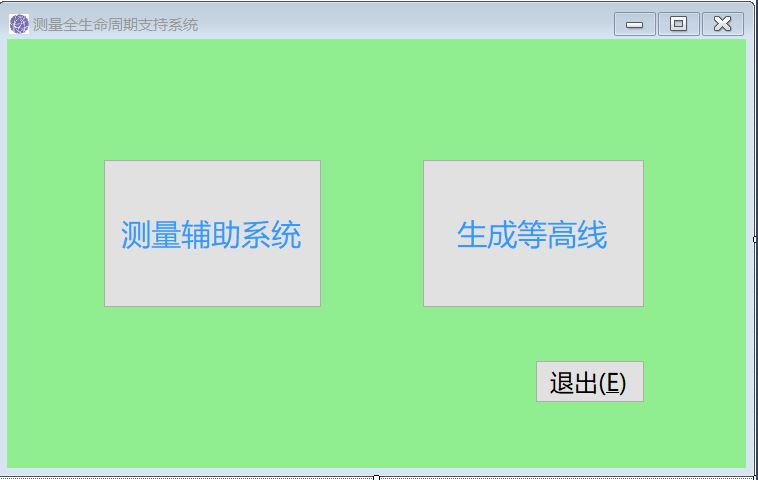
\includegraphics[width=0.8\textwidth]{mainform.JPG}
\end{figure}

第二个窗体是FormSurvey,辅助有关测量行为的进行,如图\ref{fig:forms}所示。
\begin{figure}[htbp]
\caption{FormSurvey}
\label{fig:forms}
\centering
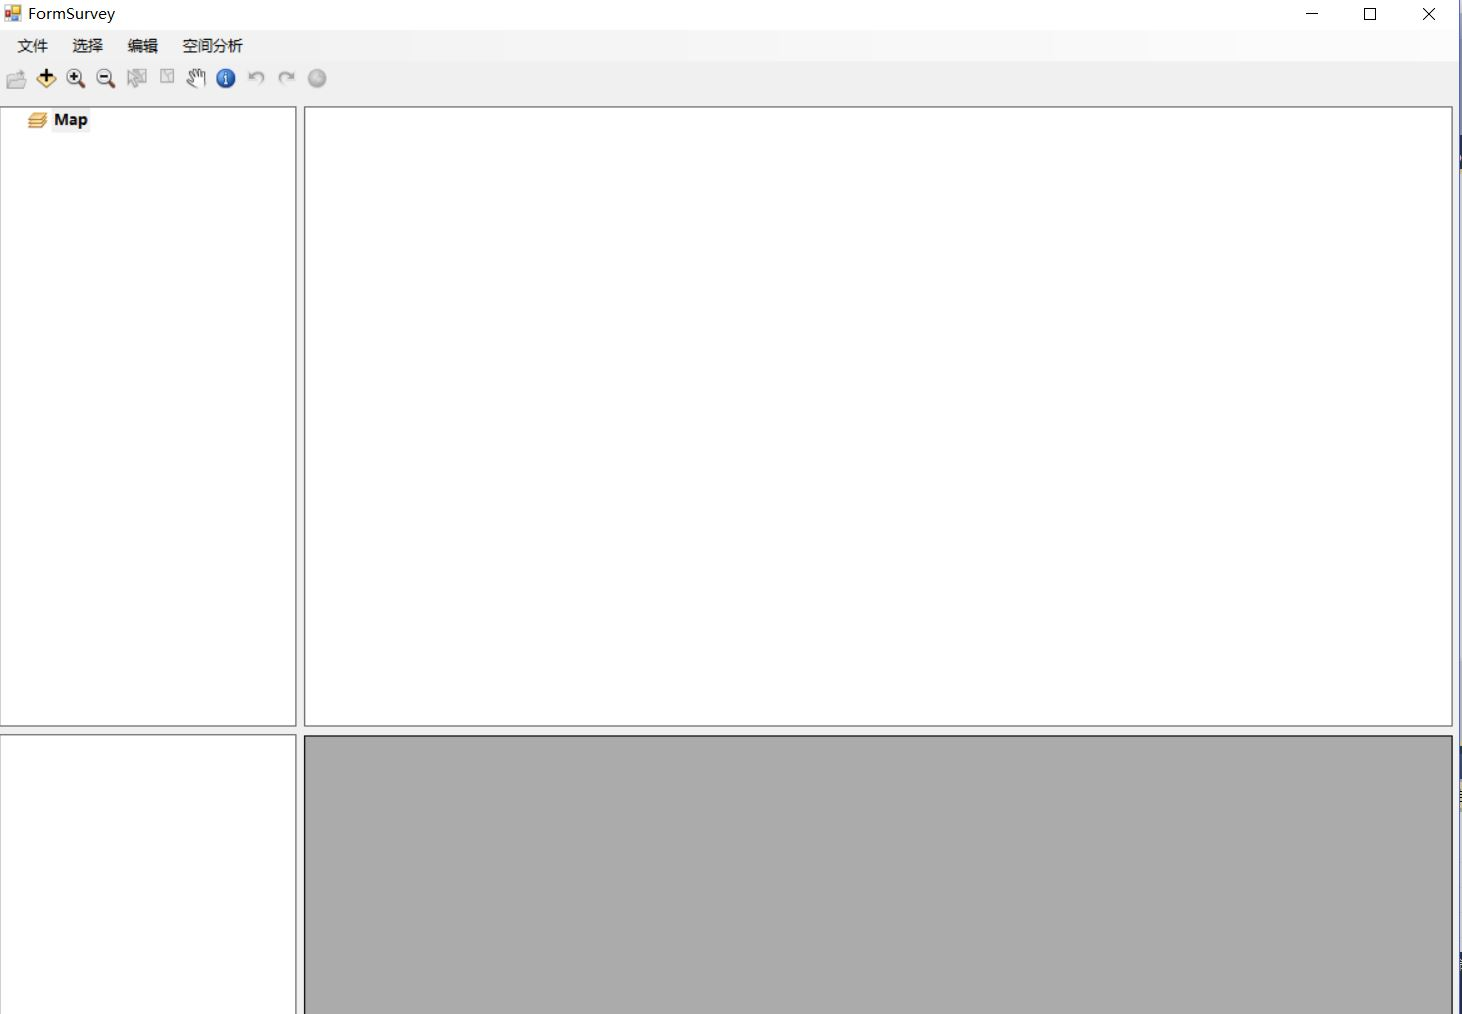
\includegraphics[width=0.8\textwidth]{forms.JPG}
\end{figure}

第三个窗体是FormCoutour,进行有关等高线的绘制,如图\ref{fig:formc}所示。
\begin{figure}[htbp]
\caption{FormCoutour}
\label{fig:formc}
\centering
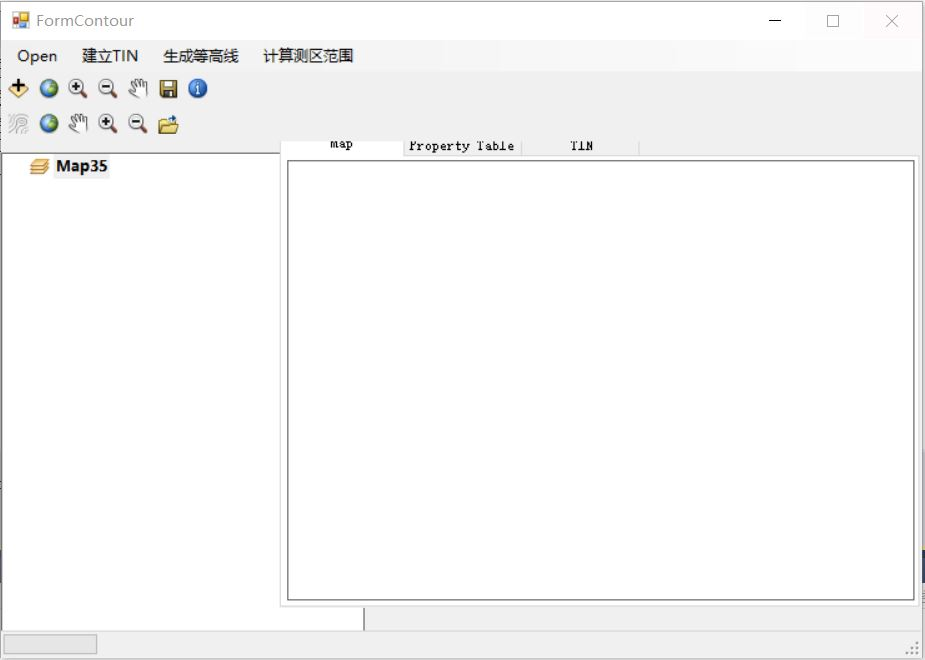
\includegraphics[width=0.8\textwidth]{formc.JPG}
\end{figure}

此外还有FormDistance,AddControlPoint等对话框。

\chapter{测量辅助系统}

测量辅助系统实现了如下特色功能
\begin{enumerate}   
\item 鹰眼功能。
\item 鼠标拖动移动图层功能。
\item 输入坐标的方式添加控制点。
\item 拉框选择测区范围,显示测区边界,并将测区范围内的控制点高亮显示。
\item 选择测站所在的控制点、输入测距,在考虑遮蔽和测距的前提下给出可用的后视点。
\item 选中测站所在的控制点,给出测区范围。
\end{enumerate}

下面分别说明这些功能
\begin{description}
\item[鹰眼功能] 利用axMapControl1的OnExtentUpdated事件,当主视图范围改变时,鹰眼视图主视图在鹰眼视图中的范围同时改变。利用axMapControl2的OnMouseDown事件,当鼠标在鹰眼视图中点击时,axMapControl1的范围同时改变。
\item[图层移动] 利用axTOCControl1的OnMouseDown事件和它的HitTest方法,记录将要移动的图层,利用OnMouseUp事件和IMap的MoveLayer方法,将其移到所属的位置。
\item[选择测区范围] 单击该选项时,将bool变量flagSelectFeature置为Checked,利用axMapControl1的OnMouseDown事件和TrackRectangle()方法,记录该选框的四个角点坐标,创建一条Polyline加入axMapControl1的图形容器中。
\item[坐标添加控制点] 单击该选项时,将弹出对话框以输入坐标,单击确定时,将该坐标保存在类GlobalData的公有静态变量中,找到点图层并添加。
\item[给出后视点] 1.点击输入仪器测量选项输入仪器测程;2.以该测程为半径生成一个缓冲区;3.选取该缓冲区内的控制点和建筑物;4.对每个除测站所在控制点之外的控制点和测站点生成一条polyline,与每个建筑物求交,若该polyline与所有建筑都不相交,则选择该控制点为后视点。
\item[给出可测范围] 选中测站所在控制点,以测程为半径并显示。
\end{description}

此外,单击图层时,可以将属性表显示在下方的dataGridView中,在TOCControl中右键单击,会弹出menuStrip,将图层上移/下移或删除。还可以在选项中添加控制点,删除控制点和(随机)修改控制点符号。

\chapter{等高线生成系统}

等高线生成系统实现了如下特色功能
\begin{enumerate}
\item 建TIN
\item TIN转栅格
\item 生成等高线
\end{enumerate}

\chapter{小组合作}

本小组的成员通过github进行合作及版本控制,方式是组长把程序推到github上,小组成员从组长的库中fork到自己的库中,更改后组长提出拉取请求(pull request),组长审核后将该提交合并(merge)到主分支。

Git版本控制系统中,将本地库叫master(主分支),将远程库叫origin。其他的分支这里还没有用到不讲。

\section{远程库}

github上提交的流程如图\ref{fig:cor}所示
\begin{figure}[htbp]
\caption{提交流程}
\label{fig:cor}
\centering
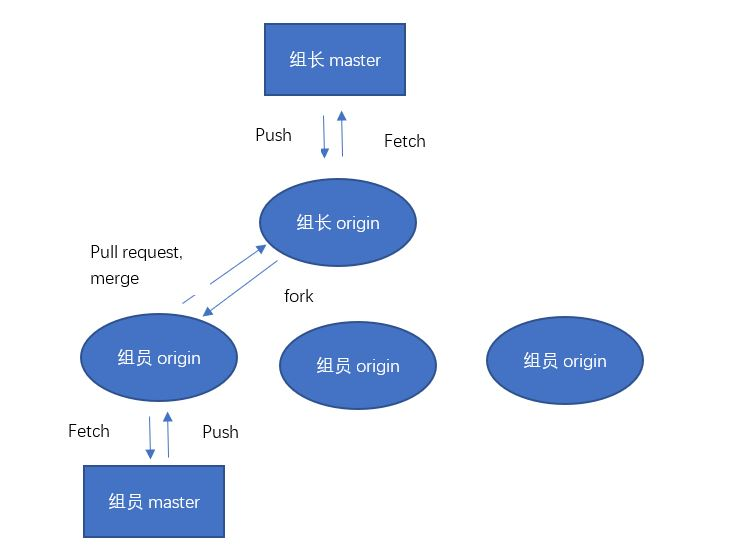
\includegraphics[width=\textwidth]{corporation.JPG}
\end{figure}

需要说明的是,因为主场的远程库在不停变动,所以组员在每次修改之前,需要先\emph{merge}组长的远程分支到master,然后才能进行修改。

\section{本地库}

下面针对本地库作讲解。在本地库中,将你选择建立git的文件夹称为工作区,add之后到暂存区,commit之后到master(主分支)。

git本地的操作如图所示\ref{fig:desktop}所示
\begin{figure}[htbp]
\caption{git本地操作}
\label{fig:desktop}
\centering
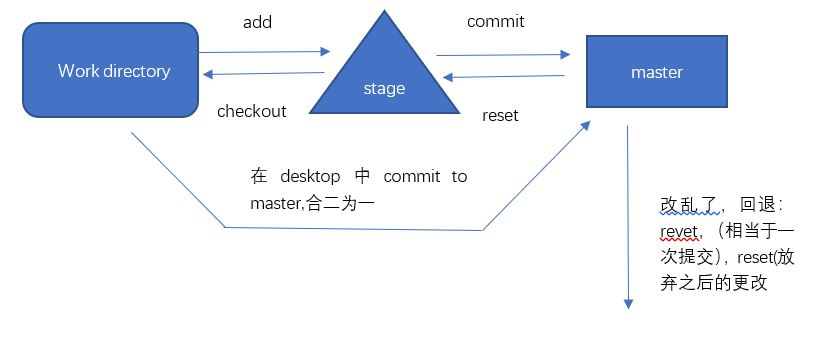
\includegraphics[width=\textwidth]{desktop.JPG}
\end{figure}

\chapter{提交文件}

\begin{table}[htbp]
\centering
\caption{文件}
\begin{tabular}{p{3cm}p{7cm}}
   项目文件 & ArcEngineProgram/ArcEngineProgram.sln  \\
    源代码 & ArcEngineProgram/ArcEngineProgram/*.cs \\
    编译好的程序 & ArcEngineProgram/ArcEngineProgram/bin/Debug/ArcEngineProgram \\
    说明文件 & document.tex,document.pdf
\end{tabular}
\end{table}

\end{document}
